\chapter{绪论}
\label{cha:intro}

\section{研究背景和意义}
\label{sec:background}
语音作为人与人之间交流最为自然的一种媒介,在我们的日常生活中起着至关重要的作用,这也使得语音一直被许多研究者认为是最有效的人机交互方式。在最近的二十年间,语音识别技术已经取得飞速的发展,它的目的是将人们说出的语音转换成对应的词序列。尽管语音识别技术已经被广泛的应用,但离真正的自然人机交互仍然有很大的距离,因为机器仍然无法准确理解说话人的情感状态并作出适当的反馈。语音中通常会包含说话人当时的情感信息,语音情感识别技术近些年受到越来越多的重视。

语音情感识别在众多自然人机交互过程中均有广泛的应用场景。在车载系统中,情感识别可以通过语音检测驾驶员当前的精神状态,并在合适的时候做出提醒从而保证驾驶安全。在心理咨询中,语音情感识别可以作为心理咨询师进行诊断的辅助工具。在同声传译系统中,语音情感识别可以通过检测说话人情感状来调整翻译内容。对于语音识别系统来说,加入情感信息同样可以提高识别准确率。在电话客服系统中,客户由于长时间的等待或者紧迫的需求,声音会变的烦躁和愤怒。在这种情况下,情感识别系统可以通过检测语音中愤怒的程度来为这些客户安排服务优先级。此外,在聊天机器人中,语音情感识别系统可以通过检测对方的情感状态来做出不同的应答。这种功能同样也可以运用在玩具中,当孩子不高兴的时候,玩具就可以通过一些方式安抚他们。在电子游戏中,尤其是在一些有语音交互的游戏中,语音情感识别可以通过模拟更加真实的交互场景来提升游戏体验。因此,语音情感识别在近几年来收到越来越多的关注。无论是在前沿模型算法的研究,还是在相关产品的落地,很多研究机构和公司都在这一领域投入大量的精力。

语音情感识别也存在许多挑战性的问题~\cite{Ayadi2011Survey, Han2014Survey}。首先,很难确定哪些声学特征与情感信息最相关。一些在语音识别领域公认的特征,例如梅尔频率倒谱系数(Mel-Frequency Cepstral Coefficients, MFCC), 在语音情感识别上并没有取得好的效果。其次,一段语音中有时会包含多种情感,如何找到每种情感对应的语音边界是个很有挑战性的问题。此外,说话人的文化背景不同,也会导致表达情感的方式上的不同,例如有的人愤怒时会说话很大声,而有的人却声音很低沉。语言同样也是影响情感表达的一个主要因素,例如汉语和德语在表达愤怒时有一些不同。还有就是情感并没有公认的规范定义,只能通过人们的主观感觉来区分,这会导致出现许多的情感类别。一些研究者倾向于一种“调色板”理论,就是只定义几种基本的情感,然后其他的情感都是由这些基本情感以不同的比例调和而成,这些基本情感被称为原型情感。最后,情感语音的数据相对来说也很难获取,这会导致许多复杂的模型无法得到充分训练。

尽管目前还没有非常成熟的语音情感识别的产品,但许多公司已经在极力推动这一领域的产品落地。Facebook早在2012年就开始进行对用户的情绪检测实验,期望能够通过情感信息来优化他们的推荐系统。微软小冰也嵌入了语音情感识别模块,希望能够和人们更自然的聊天。IBM与软银合作推出了具有情绪感知能力的机器人Pepper。苹果也开始在自己的产品中加入语音情感识别的功能。国内的公司在近几年也开始这一领域的产品化,科大讯飞公司已经开始推出语音情感识别相关的技术支持,百度视频也推出基于情感识别的内容推荐系统。此外,也有一些创业公司开始关注语音情感识别,例如竹简智能。

\section{研究现状}
\label{sec:status}
语音情感识别根据处理流程不同大致可以分为两种类型,一种是从语音信号中抽取声学特征,然后通过分类器区分情感类别的传统方法,另一种是直接将原始语音信号映射到情感类别的端到端系统,下面将分别介绍这这两类方法。

\subsection{传统的语音情感识别}
\label{ssec:classical_emo_rec}
传统的语音情感识别主要可以分为两个部分,第一部分是抽取和情感信息相关的声学特征,第二部分是使用分类器将特征向量映射到对应的情感类别,图\ref{fig:traditional_speech_emotion_recognition}是传统语音情感识别的流程图。

\begin{figure}[htb] % use float package if you want it here
    \centering
    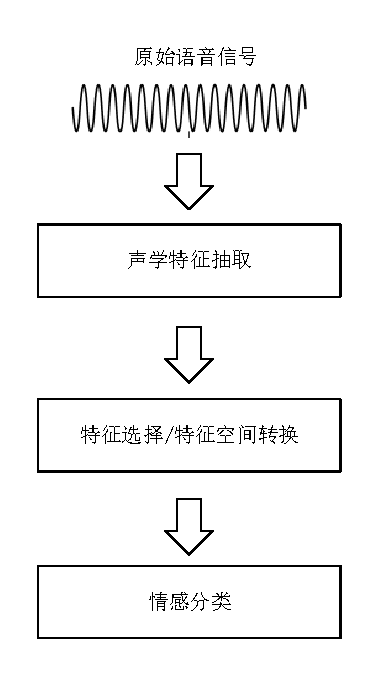
\includegraphics[height=10cm]{myfigures/traditional_speech_emotion_recognition}
    \caption{传统语音情感识别流程图}
    \label{fig:traditional_speech_emotion_recognition}
\end{figure}

特征选择是一个在所有分类问题中都存在的问题,目的是抽取与分类目标最相关的特征子集。语音情感识别作为一个分类任务,在这方面已经有很多的研究工作。首先,韵律学相关的特征已经被广泛的应用在语音情感识别中~\cite{Cowie2002Emotion, Lee2005Toward, Murray1993Toward},包括基频相关的特征,能量相关的特征和时长相关的特征。其次,谱相关的特征也在情感识别中起到了重要的作用~\cite{Atal1974Effectiveness, Banse1996Acoustic, Bou2000A, Hernando1997Linear, Kaiser1962Communication, Rabiner1999Fundamentals},例如线性预测系数(Linear Prediction Coefficients, LPC),线性预测倒谱系数(Linear Prediction Cepstral Coefficients, LPCC)以及梅尔频率倒谱系数(Mel-frequency Cepstral Coefficients, MFCC)。此外,声音质量相关的特征也被证明同情感识别任务相关~\cite{Cowie2002Emotion, Davitz1964The}。

从语音信号中抽取声学特征后,接下来就变成了一个基本的分类问题,有许多的分类模型已经被运用在情感识别任务中。隐马尔可夫模型(Hidden Markov Model, HMM)是被广泛使用在语音识别中的一种模型~\cite{Rabiner2007An, Ephraim2002Hidden, Schuller2003Hidden, Nogueiras2012Speech, Kwon2003Emotion, Lee2004Emotion},它的运作原理和语音产生的机制十分相似,因此这种模型同样也在语音情感识别中被使用。高斯混合模型(Gaussian Mixture Models, GMM)是一种概率分布模型~\cite{Vlassis2002A, Reynolds1995Robust, Rissanen1978Modeling, El2004On, Vlassis1999A, Breazeal2002Recognition, Slaney2003Baby},它使用多变量的高斯分布来预测当前语音句子属于不同情感类别的概率,在一些公开数据集上取得了不错的效果。支持向量机(Support Vector Machine, SVM)是一种被广泛使用在许多模式识别任务中的分类模型,它通过核函数(Kernel Functions)将低维空间无法区分的特征向量映射到更高维的空间,然后用线性分类器将其区分,这种模型在许多语音情感识别的研究中也被使用~\cite{Burges2008A, Schuller2004Speech, Pierre2003The}。随着计算能力和存储容量的提升,深度学习模型在近几年变得逐渐流行,在许多的任务上都超过了传统的机器学习算法。在语音情感识别领域,深度学习的方法同样也被广泛使用~\cite{Carpenter1989Neural, Nicholson2000Emotion, Crystal1978Linear, Hozjan2003Context, Petrushin2000EMOTION}。除了上面这些单独的分类模型,还有一些工作尝试将多种模型混合使用,然后共同决策最后的情感类别,期望能够提高系统的鲁棒性~\cite{Schuller2005Robust, Kuncheva2004Combining, Lugger2015Combining, Mashao2006Combining, Wu2005Linear, Kuncheva2002A}。

\subsection{端到端的语音情感识别}
\label{ssec:end2end_emo_rec}
在最近几年,深度学习的方法和工具已经被运用到语音处理领域~\cite{Han2014Speech, Lee2015High, Huang2014Speech, Le2013Emotion, Rana2016Emotion, Chernykh2017Emotion},包括用于特征抽取,分类和回归任务,或者两者兼而有之。一些实验结果显示在原始语音信号上使用深度神经网络提取特征可以比采用人工定义的声学特征得到更好的效果~\cite{Trigeorgis2016Adieu}。这导致许多的研究者开始采用端到端的系统,即省略声学特征提取的过程,直接建立从原始语音信号到任务目标的映射,图\ref{fig:end2end_speech_emotion_recognition}是端到端的语音情感识别流程图。

\begin{figure}[htb] % use float package if you want it here
    \centering
    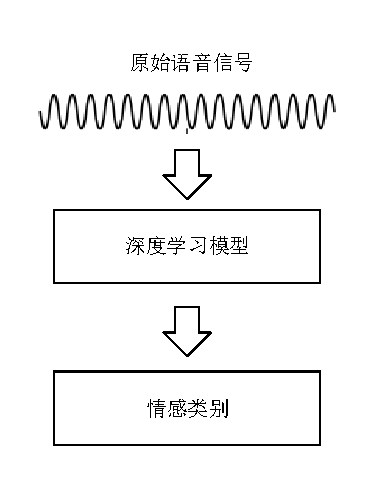
\includegraphics[height=8cm]{myfigures/end2end_speech_emotion_recognition}
    \caption{端到端语音情感识别流程图}
    \label{fig:end2end_speech_emotion_recognition}
\end{figure}

这种端到端的系统最早出现在语音识别领域,最早的工作是Jaitly等人~\cite{Jaitly2011Learning}通过受限玻尔兹曼机(Restricted Boltzmann Machine, RBM)从原始语音信号上得到一种有利于语音识别的中间表示。Bhargava等人~\cite{Bhargava2015Architectures}则是通过堆叠的全连接神经网络从原始语音信号得到瓶颈特征(Bottleneck Feature),并且取得了和使用梅尔频率倒谱系数相近的效果。 Sainath等人~\cite{Sainath2015Convolutional}将卷积神经网络(Convolution Neural Network, CNN)和长短时记忆循环神经网络(Long-Short Term Memory Recurrent Neural Network, LSTM-RNN)用在大词表语音识别上。Hannun和Amodei~\cite{Amodei2015Deep}在线性语谱图(Linearly-Spaced Spectrogram)上采用深度神经网络,搭建出了当时最好的语音识别系统。此外,在梅尔语谱图(Mel-Scale Spectrogram)上使用深度学习方法,进行说话人识别也取得了很不错的效果~\cite{Variani2014Deep}。

在语音情感识别领域也开始有一些端到端的方法被提出。George等人~\cite{Trigeorgis2016Adieu}提出一种使用CNN从原始语音信号提取特征,然后通过LSTM-RNN捕获输入序列的时序信息并最终输出不同情感的后验概率,并且发现LSTM-RNN不同节点的输出和一些声学特征有很强的相关性。Satt等人~\cite{Satt2017Efficient}也采用了相似的神经网络结构,但不同的是他们从语谱图(Spectrogram)上抽取特征而非原始语音信号。他们认为在语谱图上可以更方便的进行去噪操作,并且在公开情感语音数据集IEMOCAP上取得了超过之前最好结果(state-of-the—art)的准确率。

\section{本文的主要研究内容和贡献}
\label{sec:content_contribution}

\subsection{研究内容和各章介绍}
\label{ssec:content}
语音情感识别效果与声学特征的选取是密切相关的,抽取什么特征以及如何抽取特征最终会影响到识别率。本文会从传统的语音情感识别和端到端的语音情感识别两类方法分别研究特征抽取和选择的方法,意使最终的情感识别准确率得到提高。

 第\ref{cha:basic_konwledge}章主要介绍语音情感识别相关的基础知识,包括情感的定义,情感语音数据库,情感相关的声学特征以及情感分类模型这四个方面的内容。首先,我们介绍了两种不同的情感定义方式,并分析了各自的优缺点。接下来我们介绍了不同类型的情感语音数据库,包括他们的采集方式和标注方式。然后我们会对情感相关的声学特征做一个全面的介绍,包括特征类型,特征选择算法和深度神经网络抽取特征。最后我们会对不同的语音情感分类模型做出介绍,包括传统的机器学习模型和深度学习模型。

 第\ref{cha:emo_pair_base_framework}章介绍了基于情感对的语音情感识别框架。通过将任意两种不同的情感组成情感对,并为不同的情感对分别选择不同的特征子集构建二分类器,从而得到更精确的二分类结果。进一步,我们发现在维度情感空间中,不同情感之前的距离并不相同,距离越近表示情感之间更相似,越远表示越不相似。我们通过条件概率建模这种相似性,并且构建贝叶斯分类器来对所有情感对的输出结果做决策融合,从而得到最终的情感类别。在实验结果上我们超过了为所有情感的分类选取相同特征集的方法,同时我们的效果也优于基于决策树的分层识别框架,这种框架的设计思想和我们很相似,但我们的方法效果更好,而且当情感类别变化时更方便构建。

 第\ref{cha:end2end}章介绍了基于深度学习的端到端的情感识别方法。在这一章我们使用深度神经网络将语谱图(Spectrogram)直接映射到对应的情感类别,省略了传统语音情感识别中的声学特征抽取的步骤。我们首先将语音信号转换为语谱图,然后采用CNN直接在语谱图上抽取特征。此外,由于语音信号属于时间序列信号,因此在CNN抽取特征后将采用RNN建模输入序列的时序信息,并将最后一个时间步的输出传给后面的全连接网络,最后通过全连接网络将输入映射到每种情感的后验概率。相比于传统声学特征,采用语谱图作为输入可以取得更好的识别效果。
 
 第\ref{cha:var_len}章介绍了如何设计能够处理变长语音段的深度神经网络结构。端到端的系统通常将句子切分为多个更短的等长语音段,并给将每个语音段都标记为所属句子的情感类别,因为大多数神经网络结构更容易处理定长的输入序列。但是将句子切分成更短的等长语音段无法保证每个语音段都包含有情感信息,这会导致网络在训练时对中性语音和情感语音产生混淆。因此,我们设计了一种能够处理变长语音段的神经网络结构,通过补齐和掩码可以保证在训练和测试的过程中都不需要对语音段进行切分,这样就可以避免上面的问题。实验结果显示,变长方法在公开的情感语音数据库IEMOCAP~\cite{Busso2008IEMOCAP}上超过了定长方法得到的最好准确率。

 第\ref{cha:summary_prospect}章对本文中关于语音情感识别中声学特征的抽取和选择的相关研究成果进行了总结,同时,还对基于情感对的识别框架和基于深度学习的端到端的框架的使用前景进行了展望。

\subsection{本文主要贡献}
\label{ssec:contribution}
本文的主要贡献点有以下几个方面:

\textbf{一、提出一种基于情感对的语音情感识别框架,为不同的情感对选择不同的声学特征,并在最后的决策融合过程中引入心理学的情感空间模型,从而提升了系统的识别率。} 传统的语音情感识别系统通常为所有的情感选取相同的声学特征来完成最后的情感分类,但实验证明不同的情感和不同的声学特征的相关性并不同。针对这一问题,我们将分别为不同的情感对选取不同的特征集合,将原先的多分类问题转变为多个二分类问题,并在最后的决策融合过程中通过贝叶斯分类器引入情感空间的信息。在公开的情感语音数据集IEMOCAP上,我们方法取得了比传统的识别框架更好的准确率。

\textbf{二、构建了基于深度神经网络的端到端的语音情感识别系统,使用语谱图代替传统的声学特征,从而提升了系统的识别率。} 随着深度学习技术和工具的发展,许多的研究者开始采用深度神经网络在原始语音信号上直接构建分类或者回归模型,被称之为端到端的系统。相比于采用传统的声学特征,这种方法可以抽取到更符合任务目标的特征表示。语谱图是语音信号的一种无损表示,我们通过卷积神经网络来从语谱图上直接抽取和情感相关的特征表示,然后通过循环神经网络来建模语音信号的时序信息,最后通过全连接网络将输出映射到不同情感的后验概率。相比于采用传统的声学特征,端到端的系统能够取得更好的准确率。

\textbf{三、设计了一种能够处理变长语音段的神经网络结构来实现端到端的系统,消除了语音分段带来的中性语音和情感语音的混淆,从而提升了系统的识别率。} 在使用深度神经网络实现端到端的语音情感识别系统时,由于卷积神经网络和循环神经网络很难处理变长的输入,通常会把变长的语音句子切分成多段等长的语音段,然后将所有语音段都标记为对应句子的情感标签,但这样会导致部分中性语音段被标记为有情感。针对于这一问题,我们采用补齐和掩码的方式来处理神经网络中变长的输入序列,避免了错误标注带来了的效果变差。相对于切分等长语音段的方法,我们直接输入整个变长语音句子的方法可以在相同的数据集上取得更好的准确率。


% 苏轼(1037-1101),北宋文学家、书画家。字子瞻,号东坡居士,眉州眉山(今属四川)人
% 。苏洵子。嘉佑进士。神宗时曾任祠部员外郎,因反对王安石新法而求外职,任杭州通判,
% 知密州、徐州、湖州。后以作诗“谤讪朝廷”罪贬黄州。哲宗时任翰林学士,曾出知杭州、
% 颖州等,官至礼部尚书。后又贬谪惠州、儋州。北还后第二年病死常州。南宋时追谥文忠。
% 与父洵弟辙,合称“三苏”。在政治上属于旧党,但也有改革弊政的要求。其文汪洋恣肆,
% 明白畅达,为“唐宋八大家”之一。  其诗清新豪健,善用夸张比喻,在艺术表现方面独具
% 风格。少数诗篇也能反映民间疾苦,指责统治者的奢侈骄纵。词开豪放一派,对后代很有影
% 响。《念奴娇·赤壁怀古》、《水调歌头·丙辰中秋》传诵甚广。

% {\kaishu 坡仙擅长行书、楷书,取法李邕、徐浩、颜真卿、杨凝式,而能自创新意。用笔丰腴
%   跌宕,有天真烂漫之趣。与蔡襄、黄庭坚、米芾并称“宋四家”。能画竹,学文同,也喜
%   作枯木怪石。论画主张“神似”,认为“论画以形似,见与儿童邻”;高度评价“诗中有
%   画,画中有诗”的艺术造诣。诗文有《东坡七集》等。存世书迹有《答谢民师论文帖》、
%   《祭黄几道文》、《前赤壁赋》、《黄州寒食诗帖》等。  画迹有《枯木怪石图》、《
%   竹石图》等。}

% {\fangsong 易与天地准,故能弥纶天地之道。仰以观於天文,俯以察於地理,是故知幽明之故。原
%   始反终,故知死生之说。精气为物,游魂为变,是故知鬼神之情状。与天地相似,故不违。
%   知周乎万物,而道济天下,故不过。旁行而不流,乐天知命,故不忧。安土敦乎仁,故
%   能爱。范围天地之化而不过,曲成万物而不遗,通乎昼夜之道而知,故神无方而易无体。}

% % 非本科生一般用不到幼圆与隶书字体。需要的同学请查看 ctex 文档。
% {\ifcsname youyuan\endcsname\youyuan\else[无 \cs{youyuan} 字体。]\fi 有天地,然后
%   万物生焉。盈天地之间者,唯万物,故受之以屯;屯者盈也,屯者物之始生也。物生必蒙,
%   故受之以蒙;蒙者蒙也,物之穉也。物穉不可不养也,故受之以需;需者饮食之道也。饮
%   食必有讼,故受之以讼。讼必有众起,故受之以师;师者众也。众必有所比,故受之以比;
%   比者比也。比必有所畜也,故受之以小畜。物畜然后有礼,故受之以履。}

% {\heiti 履而泰,然后安,故受之以泰;泰者通也。物不可以终通,故受之以否。物不可以终
%   否,故受之以同人。与人同者,物必归焉,故受之以大有。有大者不可以盈,故受之以谦。
%   有大而能谦,必豫,故受之以豫。豫必有随,故受之以随。以喜随人者,必有事,故受
%   之以蛊;蛊者事也。}

% {\ifcsname lishu\endcsname\lishu\else[无 \cs{lishu} 字体。]\fi 有事而后可大,故受
%   之以临;临者大也。物大然后可观,故受之以观。可观而后有所合,故受之以噬嗑;嗑者
%   合也。物不可以苟合而已,故受之以贲;贲者饰也。致饰然后亨,则尽矣,故受之以剥;
%   剥者剥也。物不可以终尽,剥穷上反下,故受之以复。复则不妄矣,故受之以无妄。}

% {\songti 有无妄然后可畜,故受之以大畜。物畜然后可养,故受之以颐;颐者养也。不养则不
%   可动,故受之以大过。物不可以终过,故受之以坎;坎者陷也。陷必有所丽,故受之以
%   离;离者丽也。}

% \section{表格样本}
% \label{chap1:sample:table} 

% \subsection{基本表格}
% \label{sec:basictable}

% 模板中关于表格的宏包有三个:\pkg{booktabs}、\pkg{array} 和 \pkg{longtabular},命
% 令有一个 \cs{hlinewd}。三线表可以用 \pkg{booktabs} 提供
% 的 \cs{toprule}、\cs{midrule} 和 \cs{bottomrule}。它们与 \pkg{longtable} 能很好的
% 配合使用。如果表格比较简单的话可以直接用命令 \cs{hlinewd}\marg{width} 控制。
% \begin{table}[htb]
%   \centering
%   \begin{minipage}[t]{0.8\linewidth} % 如果想在表格中使用脚注,minipage是个不错的办法
%   \caption[模板文件]{模板文件。如果表格的标题很长,那么在表格索引中就会很不美
%     观,所以要像 chapter 那样在前面用中括号写一个简短的标题。这个标题会出现在索
%     引中。}
%   \label{tab:template-files}
%     \begin{tabularx}{\linewidth}{lX}
%       \toprule[1.5pt]
%       {\heiti 文件名} & {\heiti 描述} \\\midrule[1pt]
%       thuthesis.ins & \LaTeX{} 安装文件,\textsc{DocStrip}\footnote{表格中的脚注} \\
%       thuthesis.dtx & 所有的一切都在这里面\footnote{再来一个}。\\
%       thuthesis.cls & 模板类文件。\\
%       thuthesis.cfg & 模板配置文。cls 和 cfg 由前两个文件生成。\\
%       thuthesis-numeric.bst    & 参考文献 BIB\TeX\ 样式文件。\\
%       thuthesis-author-year.bst    & 参考文献 BIB\TeX\ 样式文件。\\
%       thuthesis.sty   & 常用的包和命令写在这里,减轻主文件的负担。\\
%       \bottomrule[1.5pt]
%     \end{tabularx}
%   \end{minipage}
% \end{table}

% 首先来看一个最简单的表格。表 \ref{tab:template-files} 列举了本模板主要文件及其功
% 能。请大家注意三线表中各条线对应的命令。这个例子还展示了如何在表格中正确使用脚注。
% 由于 \LaTeX{} 本身不支持在表格中使用 \cs{footnote},所以我们不得不将表格放在
% 小页中,而且最好将表格的宽度设置为小页的宽度,这样脚注看起来才更美观。

% \subsection{复杂表格}
% \label{sec:complicatedtable}

% 我们经常会在表格下方标注数据来源,或者对表格里面的条目进行解释。前面的脚注是一种
% 不错的方法,如果不喜欢脚注,可以在表格后面写注释,比如表~\ref{tab:tabexamp1}。
% \begin{table}[htbp]
%   \centering
%   \caption{复杂表格示例 1}
%   \label{tab:tabexamp1}
%   \begin{minipage}[t]{0.8\textwidth} 
%     \begin{tabularx}{\linewidth}{|l|X|X|X|X|}
%       \hline
%       \multirow{2}*{\diagbox[width=5em]{x}{y}} & \multicolumn{2}{c|}{First Half} & \multicolumn{2}{c|}{Second Half}\\\cline{2-5}
%       & 1st Qtr &2nd Qtr&3rd Qtr&4th Qtr \\ \hline
%       East$^{*}$ &   20.4&   27.4&   90&     20.4 \\
%       West$^{**}$ &   30.6 &   38.6 &   34.6 &  31.6 \\ \hline
%     \end{tabularx}\\[2pt]
%     \footnotesize 注:数据来源《\thuthesis{} 使用手册》。\\
%     *:东部\\
%     **:西部
%   \end{minipage}
% \end{table}

% 此外,表~\ref{tab:tabexamp1} 同时还演示了另外两个功能:1)通过 \pkg{tabularx} 的
%  \texttt{|X|} 扩展实现表格自动放大;2)通过命令 \cs{diagbox} 在表头部分
% 插入反斜线。

% 为了使我们的例子更接近实际情况,我会在必要的时候插入一些“无关”文字,以免太多图
% 表同时出现,导致排版效果不太理想。第一个出场的当然是我的最爱:风流潇洒、骏马绝尘、
% 健笔凌云的{\heiti 李太白}了。

% 李白,字太白,陇西成纪人。凉武昭王暠九世孙。或曰山东人,或曰蜀人。白少有逸才,志
% 气宏放,飘然有超世之心。初隐岷山,益州长史苏颋见而异之,曰:“是子天才英特,可比
% 相如。”天宝初,至长安,往见贺知章。知章见其文,叹曰:“子谪仙人也。”言于明皇,
% 召见金銮殿,奏颂一篇。帝赐食,亲为调羹,有诏供奉翰林。白犹与酒徒饮于市,帝坐沉香
% 亭子,意有所感,欲得白为乐章,召入,而白已醉。左右以水颒面,稍解,援笔成文,婉丽
% 精切。帝爱其才,数宴见。白常侍帝,醉,使高力士脱靴。力士素贵,耻之,摘其诗以激杨
% 贵妃。帝欲官白,妃辄沮止。白自知不为亲近所容,恳求还山。帝赐金放还。乃浪迹江湖,
% 终日沉饮。永王璘都督江陵,辟为僚佐。璘谋乱,兵败,白坐长流夜郎,会赦得还。族人阳
% 冰为当涂令,白往依之。代宗立,以左拾遗召,而白已卒。文宗时,诏以白歌诗、裴旻剑舞、
% 张旭草书为三绝云。集三十卷。今编诗二十五卷。\hfill —— 《全唐诗》诗人小传

% 浮动体的并排放置一般有两种情况:1)二者没有关系,为两个独立的浮动体;2)二者隶属
% 于同一个浮动体。对表格来说并排表格既可以像图~\ref{tab:parallel1}、
% 图~\ref{tab:parallel2} 使用小页环境,也可以如图~\ref{tab:subtable} 使用子表格来做。
% 图的例子参见第~\ref{sec:multifig} 节。

% \begin{table}[htbp]
% \noindent\begin{minipage}{0.5\textwidth}
% \centering
% \caption{第一个并排子表格}
% \label{tab:parallel1}
% \begin{tabular}{p{2cm}p{2cm}}
% \toprule[1.5pt]
% 111 & 222 \\\midrule[1pt]
% 222 & 333 \\\bottomrule[1.5pt]
% \end{tabular}
% \end{minipage}%
% \begin{minipage}{0.5\textwidth}
% \centering
% \caption{第二个并排子表格}
% \label{tab:parallel2}
% \begin{tabular}{p{2cm}p{2cm}}
% \toprule[1.5pt]
% 111 & 222 \\\midrule[1pt]
% 222 & 333 \\\bottomrule[1.5pt]
% \end{tabular}
% \end{minipage}
% \end{table}

% 然后就是忧国忧民,诗家楷模杜工部了。杜甫,字子美,其先襄阳人,曾祖依艺为巩令,因
% 居巩。甫天宝初应进士,不第。后献《三大礼赋》,明皇奇之,召试文章,授京兆府兵曹参
% 军。安禄山陷京师,肃宗即位灵武,甫自贼中遁赴行在,拜左拾遗。以论救房琯,出为华州
% 司功参军。关辅饥乱,寓居同州同谷县,身自负薪采梠,餔糒不给。久之,召补京兆府功曹,
% 道阻不赴。严武镇成都,奏为参谋、检校工部员外郎,赐绯。武与甫世旧,待遇甚厚。乃于
% 成都浣花里种竹植树,枕江结庐,纵酒啸歌其中。武卒,甫无所依,乃之东蜀就高適。既至
% 而適卒。是岁,蜀帅相攻杀,蜀大扰。甫携家避乱荆楚,扁舟下峡,未维舟而江陵亦乱。乃
% 溯沿湘流,游衡山,寓居耒阳。卒年五十九。元和中,归葬偃师首阳山,元稹志其墓。天宝
% 间,甫与李白齐名,时称李杜。然元稹之言曰:“李白壮浪纵恣,摆去拘束,诚亦差肩子美
% 矣。至若铺陈终始,排比声韵,大或千言,次犹数百,词气豪迈,而风调清深,属对律切,
% 而脱弃凡近,则李尚不能历其藩翰,况堂奥乎。”白居易亦云:“杜诗贯穿古今,  尽工尽
% 善,殆过于李。”元、白之论如此。盖其出处劳佚,喜乐悲愤,好贤恶恶,一见之于诗。而
% 又以忠君忧国、伤时念乱为本旨。读其诗可以知其世,故当时谓之“诗史”。旧集诗文共六
% 十卷,今编诗十九卷。

% \begin{table}[htbp]
% \centering
% \caption{并排子表格}
% \label{tab:subtable}
% \subcaptionbox{第一个子表格}
% {
% \begin{tabular}{p{2cm}p{2cm}}
% \toprule[1.5pt]
% 111 & 222 \\\midrule[1pt]
% 222 & 333 \\\bottomrule[1.5pt]
% \end{tabular}
% }
% \hskip2cm
% \subcaptionbox{第二个子表格}
% {
% \begin{tabular}{p{2cm}p{2cm}}
% \toprule[1.5pt]
% 111 & 222 \\\midrule[1pt]
% 222 & 333 \\\bottomrule[1.5pt]
% \end{tabular}
% }
% \end{table}

% 不可否认 \LaTeX{} 的表格功能没有想象中的那么强大,不过只要足够认真,足够细致,
% 同样可以排出来非常复杂非常漂亮的表格。请参看表~\ref{tab:tabexamp2}。
% \begin{table}[htbp]
%   \centering\dawu[1.3]
%   \caption{复杂表格示例 2}
%   \label{tab:tabexamp2}
%   \begin{tabular}[c]{|m{1.5cm}|c|c|c|c|c|c|}\hline
%     \multicolumn{2}{|c|}{Network Topology} & \# of nodes & 
%     \multicolumn{3}{c|}{\# of clients} & Server \\\hline
%     GT-ITM & Waxman Transit-Stub & 600 &
%     \multirow{2}{2em}{2\%}& 
%     \multirow{2}{2em}{10\%}& 
%     \multirow{2}{2em}{50\%}& 
%     \multirow{2}{1.2in}{Max. Connectivity}\\\cline{1-3}
%     \multicolumn{2}{|c|}{Inet-2.1} & 6000 & & & &\\\hline
%     \multirow{2}{1.5cm}{Xue} & Rui  & Ni &\multicolumn{4}{c|}{\multirow{2}*{\thuthesis}}\\\cline{2-3}
%     & \multicolumn{2}{c|}{ABCDEF} &\multicolumn{4}{c|}{} \\\hline
% \end{tabular}
% \end{table}

% 最后就是清新飘逸、文约意赅、空谷绝响的王大侠了。王维,字摩诘,河东人。工书画,与
% 弟缙俱有俊才。开元九年,进士擢第,调太乐丞。坐累为济州司仓参军,历右拾遗、监察御
% 史、左补阙、库部郎中,拜吏部郎中。天宝末,为给事中。安禄山陷两都,维为贼所得,服
% 药阳喑,拘于菩提寺。禄山宴凝碧池,维潜赋诗悲悼,闻于行在。贼平,陷贼官三等定罪,
% 特原之,责授太子中允,迁中庶子、中书舍人。复拜给事中,转尚书右丞。维以诗名盛于开
% 元、天宝间,宁薛诸王驸马豪贵之门,无不拂席迎之。得宋之问辋川别墅,山水绝胜,与道
% 友裴迪,浮舟往来,弹琴赋诗,啸咏终日。笃于奉佛,晚年长斋禅诵。一日,忽索笔作书
% 数纸,别弟缙及平生亲故,舍笔而卒。赠秘书监。宝应中,代宗问缙:“朕常于诸王坐闻维
% 乐章,今存几何?”缙集诗六卷,文四卷,表上之。敕答云,卿伯氏位列先朝,名高希代。
% 抗行周雅,长揖楚辞。诗家者流,时论归美。克成编录,叹息良深。殷璠谓维诗词秀调雅,
% 意新理惬。在泉成珠,著壁成绘。苏轼亦云:“维诗中有画,画中有诗也。”今编诗四卷。

% 要想用好论文模板还是得提前学习一些 \TeX/\LaTeX{}的相关知识,具备一些基本能力,掌
% 握一些常见技巧,否则一旦遇到问题还真是比较麻烦。我们见过很多这样的同学,一直以来
% 都是使用 Word 等字处理工具,以为 \LaTeX{}模板的用法也应该类似,所以就沿袭同样的思
% 路来对待这种所见非所得的排版工具,结果被折腾的焦头烂额,疲惫不堪。

% 如果您要排版的表格长度超过一页,那么推荐使用 \pkg{longtable} 或者 \pkg{supertabular}
% 宏包,模板对 \pkg{longtable} 进行了相应的设置,所以用起来可能简单一些。
% 表~\ref{tab:performance} 就是 \pkg{longtable} 的简单示例。
% \begin{longtable}[c]{c*{6}{r}}
% \caption{实验数据}\label{tab:performance}\\
% \toprule[1.5pt]
%  测试程序 & \multicolumn{1}{c}{正常运行} & \multicolumn{1}{c}{同步} & \multicolumn{1}{c}{检查点} & \multicolumn{1}{c}{卷回恢复}
% & \multicolumn{1}{c}{进程迁移} & \multicolumn{1}{c}{检查点} \\
% & \multicolumn{1}{c}{时间 (s)}& \multicolumn{1}{c}{时间 (s)}&
% \multicolumn{1}{c}{时间 (s)}& \multicolumn{1}{c}{时间 (s)}& \multicolumn{1}{c}{
%   时间 (s)}&  文件(KB)\\\midrule[1pt]
% \endfirsthead
% \multicolumn{7}{c}{续表~\thetable\hskip1em 实验数据}\\
% \toprule[1.5pt]
%  测试程序 & \multicolumn{1}{c}{正常运行} & \multicolumn{1}{c}{同步} & \multicolumn{1}{c}{检查点} & \multicolumn{1}{c}{卷回恢复}
% & \multicolumn{1}{c}{进程迁移} & \multicolumn{1}{c}{检查点} \\
% & \multicolumn{1}{c}{时间 (s)}& \multicolumn{1}{c}{时间 (s)}&
% \multicolumn{1}{c}{时间 (s)}& \multicolumn{1}{c}{时间 (s)}& \multicolumn{1}{c}{
%   时间 (s)}&  文件(KB)\\\midrule[1pt]
% \endhead
% \hline
% \multicolumn{7}{r}{续下页}
% \endfoot
% \endlastfoot
% CG.A.2 & 23.05 & 0.002 & 0.116 & 0.035 & 0.589 & 32491 \\
% CG.A.4 & 15.06 & 0.003 & 0.067 & 0.021 & 0.351 & 18211 \\
% CG.A.8 & 13.38 & 0.004 & 0.072 & 0.023 & 0.210 & 9890 \\
% CG.B.2 & 867.45 & 0.002 & 0.864 & 0.232 & 3.256 & 228562 \\
% CG.B.4 & 501.61 & 0.003 & 0.438 & 0.136 & 2.075 & 123862 \\
% CG.B.8 & 384.65 & 0.004 & 0.457 & 0.108 & 1.235 & 63777 \\
% MG.A.2 & 112.27 & 0.002 & 0.846 & 0.237 & 3.930 & 236473 \\
% MG.A.4 & 59.84 & 0.003 & 0.442 & 0.128 & 2.070 & 123875 \\
% MG.A.8 & 31.38 & 0.003 & 0.476 & 0.114 & 1.041 & 60627 \\
% MG.B.2 & 526.28 & 0.002 & 0.821 & 0.238 & 4.176 & 236635 \\
% MG.B.4 & 280.11 & 0.003 & 0.432 & 0.130 & 1.706 & 123793 \\
% MG.B.8 & 148.29 & 0.003 & 0.442 & 0.116 & 0.893 & 60600 \\
% LU.A.2 & 2116.54 & 0.002 & 0.110 & 0.030 & 0.532 & 28754 \\
% LU.A.4 & 1102.50 & 0.002 & 0.069 & 0.017 & 0.255 & 14915 \\
% LU.A.8 & 574.47 & 0.003 & 0.067 & 0.016 & 0.192 & 8655 \\
% LU.B.2 & 9712.87 & 0.002 & 0.357 & 0.104 & 1.734 & 101975 \\
% LU.B.4 & 4757.80 & 0.003 & 0.190 & 0.056 & 0.808 & 53522 \\
% LU.B.8 & 2444.05 & 0.004 & 0.222 & 0.057 & 0.548 & 30134 \\
% EP.A.2 & 123.81 & 0.002 & 0.010 & 0.003 & 0.074 & 1834 \\
% EP.A.4 & 61.92 & 0.003 & 0.011 & 0.004 & 0.073 & 1743 \\
% EP.A.8 & 31.06 & 0.004 & 0.017 & 0.005 & 0.073 & 1661 \\
% EP.B.2 & 495.49 & 0.001 & 0.009 & 0.003 & 0.196 & 2011 \\
% EP.B.4 & 247.69 & 0.002 & 0.012 & 0.004 & 0.122 & 1663 \\
% EP.B.8 & 126.74 & 0.003 & 0.017 & 0.005 & 0.083 & 1656 \\
% \bottomrule[1.5pt]
% \end{longtable}

% \subsection{其它}
% \label{sec:tableother}
% 如果不想让某个表格或者图片出现在索引里面,请使用命令 \cs{caption*}。
% 这个命令不会给表格编号,也就是出来的只有标题文字而没有“表~XX”,“图~XX”,否则
% 索引里面序号不连续就显得不伦不类,这也是 \LaTeX{} 里星号命令默认的规则。

% 有这种需求的多是本科同学的英文资料翻译部分,如果觉得附录中英文原文中的表格和图
% 片显示成“表”和“图”不协调的话,一个很好的办法就是用 \cs{caption*},参数
% 随便自己写,比如不守规矩的表~1.111 和图~1.111 能满足这种特殊需要(可以参看附录部
% 分)。
% \begin{table}[ht]
%   \begin{minipage}{0.4\linewidth}
%     \centering
%     \caption*{表~1.111\quad 这是一个手动编号,不出现在索引中的表格。}
%     \label{tab:badtabular}
%       \framebox(150,50)[c]{\thuthesis}
%   \end{minipage}%
%   \hfill%
%   \begin{minipage}{0.4\linewidth}
%     \centering
%     \caption*{Figure~1.111\quad 这是一个手动编号,不出现在索引中的图。}
%     \label{tab:badfigure}
%     \framebox(150,50)[c]{薛瑞尼}
%   \end{minipage}
% \end{table}

% 如果的确想让它编号,但又不想让它出现在索引中的话,目前模板上不支持。

% 最后,虽然大家不一定会独立使用小页,但是关于小页中的脚注还是有必要提一下。请看下
% 面的例子。

% \begin{minipage}[t]{\linewidth-2\parindent}
%   柳宗元,字子厚(773-819),河东(今永济县)人\footnote{山西永济水饺。},是唐代
%   杰出的文学家,哲学家,同时也是一位政治改革家。与韩愈共同倡导唐代古文运动,并称
%   韩柳\footnote{唐宋八大家之首二位。}。
% \end{minipage}

% 唐朝安史之乱后,宦官专权,藩镇割据,土地兼并日渐严重,社会生产破坏严重,民不聊生。柳宗
% 元对这种社会现实极为不满,他积极参加了王叔文领导的“永济革新”,并成为这一
% 运动的中坚人物。他们革除弊政,打击权奸,触犯了宦官和官僚贵族利益,在他们的联合反
% 扑下,改革失败了,柳宗元被贬为永州司马。

% \section{定理环境}
% \label{sec:theorem}

% 给大家演示一下各种和证明有关的环境:

% \begin{assumption}
% 待月西厢下,迎风户半开;隔墙花影动,疑是玉人来。
% \begin{eqnarray}
%   \label{eq:eqnxmp}
%   c & = & a^2 - b^2\\
%     & = & (a+b)(a-b)
% \end{eqnarray}
% \end{assumption}

% 千辛万苦,历尽艰难,得有今日。然相从数千里,未曾哀戚。今将渡江,方图百年欢笑,如
% 何反起悲伤?(引自《杜十娘怒沉百宝箱》)

% \begin{definition}
% 子曰:「道千乘之国,敬事而信,节用而爱人,使民以时。」
% \end{definition}

% 千古第一定义!问世间、情为何物,只教生死相许?天南地北双飞客,老翅几回寒暑。欢乐趣,离别苦,就中更有痴儿女。
% 君应有语,渺万里层云,千山暮雪,只影向谁去?

% 横汾路,寂寞当年箫鼓,荒烟依旧平楚。招魂楚些何嗟及,山鬼暗谛风雨。天也妒,未信与,莺儿燕子俱黄土。
% 千秋万古,为留待骚人,狂歌痛饮,来访雁丘处。

% \begin{proposition}
%  曾子曰:「吾日三省吾身 —— 为人谋而不忠乎?与朋友交而不信乎?传不习乎?」
% \end{proposition}

% 多么凄美的命题啊!其日牛马嘶,新妇入青庐,奄奄黄昏后,寂寂人定初,我命绝今日,
% 魂去尸长留,揽裙脱丝履,举身赴清池,府吏闻此事,心知长别离,徘徊庭树下,自挂东南
% 枝。

% \begin{remark}
% 天不言自高,水不言自流。
% \begin{gather*}
% \begin{split} 
% \varphi(x,z)
% &=z-\gamma_{10}x-\gamma_{mn}x^mz^n\\
% &=z-Mr^{-1}x-Mr^{-(m+n)}x^mz^n
% \end{split}\\[6pt]
% \begin{align} \zeta^0&=(\xi^0)^2,\\
% \zeta^1 &=\xi^0\xi^1,\\
% \zeta^2 &=(\xi^1)^2,
% \end{align}
% \end{gather*}
% \end{remark}

% 天尊地卑,乾坤定矣。卑高以陈,贵贱位矣。 动静有常,刚柔断矣。方以类聚,物以群分,
% 吉凶生矣。在天成象,在地成形,变化见矣。鼓之以雷霆,润之以风雨,日月运行,一寒一
% 暑,乾道成男,坤道成女。乾知大始,坤作成物。乾以易知,坤以简能。易则易知,简则易
% 从。易知则有亲,易从则有功。有亲则可久,有功则可大。可久则贤人之德,可大则贤人之
% 业。易简,而天下矣之理矣;天下之理得,而成位乎其中矣。

% \begin{axiom}
% 两点间直线段距离最短。  
% \begin{align}
% x&\equiv y+1\pmod{m^2}\\
% x&\equiv y+1\mod{m^2}\\
% x&\equiv y+1\pod{m^2}
% \end{align}
% \end{axiom}

% 《彖曰》:大哉乾元,万物资始,乃统天。云行雨施,品物流形。大明始终,六位时成,时
% 乘六龙以御天。乾道变化,各正性命,保合大和,乃利贞。首出庶物,万国咸宁。

% 《象曰》:天行健,君子以自强不息。潜龙勿用,阳在下也。见龙再田,德施普也。终日乾
% 乾,反复道也。或跃在渊,进无咎也。飞龙在天,大人造也。亢龙有悔,盈不可久也。用九,
% 天德不可为首也。   

% \begin{lemma}
% 《猫和老鼠》是我最爱看的动画片。
% \begin{multline*}%\tag*{[a]} % 这个不出现在索引中
% \int_a^b\biggl\{\int_a^b[f(x)^2g(y)^2+f(y)^2g(x)^2]
%  -2f(x)g(x)f(y)g(y)\,dx\biggr\}\,dy \\
%  =\int_a^b\biggl\{g(y)^2\int_a^bf^2+f(y)^2
%   \int_a^b g^2-2f(y)g(y)\int_a^b fg\biggr\}\,dy
% \end{multline*}
% \end{lemma}

% 行行重行行,与君生别离。相去万余里,各在天一涯。道路阻且长,会面安可知。胡马依北
% 风,越鸟巢南枝。相去日已远,衣带日已缓。浮云蔽白日,游子不顾返。思君令人老,岁月
% 忽已晚。  弃捐勿复道,努力加餐饭。

% \begin{theorem}\label{the:theorem1}
% 犯我强汉者,虽远必诛\hfill —— 陈汤(汉)
% \end{theorem}
% \begin{subequations}
% \begin{align}
% y & = 1 \\
% y & = 0
% \end{align}
% \end{subequations}
% 道可道,非常道。名可名,非常名。无名天地之始;有名万物之母。故常无,欲以观其妙;
% 常有,欲以观其徼。此两者,同出而异名,同谓之玄。玄之又玄,众妙之门。上善若水。水
% 善利万物而不争,处众人之所恶,故几于道。曲则全,枉则直,洼则盈,敝则新,少则多,
% 多则惑。人法地,地法天,天法道,道法自然。知人者智,自知者明。胜人者有力,自胜
% 者强。知足者富。强行者有志。不失其所者久。死而不亡者寿。

% \begin{proof}
% 燕赵古称多感慨悲歌之士。董生举进士,连不得志于有司,怀抱利器,郁郁适兹土,吾
% 知其必有合也。董生勉乎哉?

% 夫以子之不遇时,苟慕义强仁者,皆爱惜焉,矧燕、赵之士出乎其性者哉!然吾尝闻
% 风俗与化移易,吾恶知其今不异于古所云邪?聊以吾子之行卜之也。董生勉乎哉?

% 吾因子有所感矣。为我吊望诸君之墓,而观于其市,复有昔时屠狗者乎?为我谢
% 曰:“明天子在上,可以出而仕矣!” \hfill —— 韩愈《送董邵南序》
% \end{proof}

% \begin{corollary}
%   四川话配音的《猫和老鼠》是世界上最好看最好听最有趣的动画片。
% \begin{alignat}{3}
% V_i & =v_i - q_i v_j, & \qquad X_i & = x_i - q_i x_j,
%  & \qquad U_i & = u_i,
%  \qquad \text{for $i\ne j$;}\label{eq:B}\\
% V_j & = v_j, & \qquad X_j & = x_j,
%   & \qquad U_j & u_j + \sum_{i\ne j} q_i u_i.
% \end{alignat}
% \end{corollary}

% 迢迢牵牛星,皎皎河汉女。
% 纤纤擢素手,札札弄机杼。
% 终日不成章,泣涕零如雨。
% 河汉清且浅,相去复几许。
% 盈盈一水间,脉脉不得语。

% \begin{example}
%   大家来看这个例子。
% \begin{equation}
% \label{ktc}
% \left\{\begin{array}{l}
% \nabla f({\mbox{\boldmath $x$}}^*)-\sum\limits_{j=1}^p\lambda_j\nabla g_j({\mbox{\boldmath $x$}}^*)=0\\[0.3cm]
% \lambda_jg_j({\mbox{\boldmath $x$}}^*)=0,\quad j=1,2,\cdots,p\\[0.2cm]
% \lambda_j\ge 0,\quad j=1,2,\cdots,p.
% \end{array}\right.
% \end{equation}
% \end{example}

% \begin{exercise}
%   请列出 Andrew S. Tanenbaum 和 W. Richard Stevens 的所有著作。
% \end{exercise}

% \begin{conjecture} \textit{Poincare Conjecture} If in a closed three-dimensional
%   space, any closed curves can shrink to a point continuously, this space can be
%   deformed to a sphere.
% \end{conjecture}

% \begin{problem}
%  回答还是不回答,是个问题。 
% \end{problem}

% 如何引用定理~\ref{the:theorem1} 呢?加上 \cs{label} 使用 \cs{ref} 即可。妾发
% 初覆额,折花门前剧。郎骑竹马来,绕床弄青梅。同居长干里,两小无嫌猜。 十四为君妇,
% 羞颜未尝开。低头向暗壁,千唤不一回。十五始展眉,愿同尘与灰。常存抱柱信,岂上望夫
% 台。 十六君远行,瞿塘滟滪堆。五月不可触,猿声天上哀。门前迟行迹,一一生绿苔。苔深
% 不能扫,落叶秋风早。八月蝴蝶来,双飞西园草。感此伤妾心,坐愁红颜老。

% \section{参考文献}
% \label{sec:bib}
% 当然参考文献可以直接写 \cs{bibitem},虽然费点功夫,但是好控制,各种格式可以自己随意改
% 写。

% 本模板推荐使用 BIB\TeX,分别提供数字引用(\texttt{thuthesis-numeric.bst})和作
% 者年份引用(\texttt{thuthesis-author-year.bst})样式,基本符合学校的参考文献格式
% (如专利等引用未加详细测试)。看看这个例子,关于书的~\cite{tex, companion,
%   ColdSources},还有这些~\cite{Krasnogor2004e, clzs, zjsw},关于杂志
% 的~\cite{ELIDRISSI94, MELLINGER96, SHELL02},硕士论文~\cite{zhubajie,
%   metamori2004},博士论文~\cite{shaheshang, FistSystem01},标准文
% 件~\cite{IEEE-1363},会议论文~\cite{DPMG,kocher99},技术报告~\cite{NPB2},电子文
% 献~\cite{chuban2001,oclc2000}。中文参考文献~\cite{cnarticle}应增
% 加 \texttt{lang=``zh''} 字段,以便进行相应处理。另外,本模板对中文文
% 献~\cite{cnproceed}的支持并不是十全十美,如果有不如意的地方,请手动修
% 改 \texttt{bbl} 文件。

% 有时候不想要上标,那么可以这样~\inlinecite{shaheshang},这个非常重要。

% 有时候一些参考文献没有纸质出处,需要标注 URL。缺省情况下,URL 不会在连字符处断行,
% 这可能使得用连字符代替空格的网址分行很难看。如果需要,可以将模板类文件中
% \begin{verbatim}
% \RequirePackage{hyperref}
% \end{verbatim}
% 一行改为:
% \begin{verbatim}
% \PassOptionsToPackage{hyphens}{url}
% \RequirePackage{hyperref}
% \end{verbatim}
% 使得连字符处可以断行。更多设置可以参考 \texttt{url} 宏包文档。

% \section{公式}
% \label{sec:equation}
% 贝叶斯公式如式~(\ref{equ:chap1:bayes}),其中 $p(y|\mathbf{x})$ 为后验;
% $p(\mathbf{x})$ 为先验;分母 $p(\mathbf{x})$ 为归一化因子。
% \begin{equation}
% \label{equ:chap1:bayes}
% p(y|\mathbf{x}) = \frac{p(\mathbf{x},y)}{p(\mathbf{x})}=
% \frac{p(\mathbf{x}|y)p(y)}{p(\mathbf{x})} 
% \end{equation}

% 论文里面公式越多,\TeX{} 就越 happy。再看一个 \pkg{amsmath} 的例子:
% \newcommand{\envert}[1]{\left\lvert#1\right\rvert} 
% \begin{equation}\label{detK2}
% \det\mathbf{K}(t=1,t_1,\dots,t_n)=\sum_{I\in\mathbf{n}}(-1)^{\envert{I}}
% \prod_{i\in I}t_i\prod_{j\in I}(D_j+\lambda_jt_j)\det\mathbf{A}
% ^{(\lambda)}(\overline{I}|\overline{I})=0.
% \end{equation} 

% 前面定理示例部分列举了很多公式环境,可以说把常见的情况都覆盖了,大家在写公式的时
% 候一定要好好看 \pkg{amsmath} 的文档,并参考模板中的用法:
% \begin{multline*}%\tag{[b]} % 这个出现在索引中的
% \int_a^b\biggl\{\int_a^b[f(x)^2g(y)^2+f(y)^2g(x)^2]
%  -2f(x)g(x)f(y)g(y)\,dx\biggr\}\,dy \\
%  =\int_a^b\biggl\{g(y)^2\int_a^bf^2+f(y)^2
%   \int_a^b g^2-2f(y)g(y)\int_a^b fg\biggr\}\,dy
% \end{multline*}

% 其实还可以看看这个多级规划:
% \begin{equation}\label{bilevel}
% \left\{\begin{array}{l}
% \max\limits_{{\mbox{\footnotesize\boldmath $x$}}} F(x,y_1^*,y_2^*,\cdots,y_m^*)\\[0.2cm]
% \mbox{subject to:}\\[0.1cm]
% \qquad G(x)\le 0\\[0.1cm]
% \qquad(y_1^*,y_2^*,\cdots,y_m^*)\mbox{ solves problems }(i=1,2,\cdots,m)\\[0.1cm]
% \qquad\left\{\begin{array}{l}
%     \max\limits_{{\mbox{\footnotesize\boldmath $y_i$}}}f_i(x,y_1,y_2,\cdots,y_m)\\[0.2cm]
%     \mbox{subject to:}\\[0.1cm]
%     \qquad g_i(x,y_1,y_2,\cdots,y_m)\le 0.
%     \end{array}\right.
% \end{array}\right.
% \end{equation}
% 这些跟规划相关的公式都来自于刘宝碇老师《不确定规划》的课件。
